\documentclass[hyperref={pdftex,unicode}]{beamer}

\usepackage[T2A]{fontenc}
\usepackage[utf8]{inputenc}
\usepackage[russian]{babel}
\usepackage{cmap}

\usepackage{xcolor}

% \usepackage{helvet}
\usepackage{pscyr}

\usepackage{multicol}

% \usepackage{amssymb,amsfonts,amsmath,mathtext}
% \usepackage{cite,enumerate,float}

\usepackage{listings}

\graphicspath{{images/}}
\usetheme{boxes}
\usecolortheme{whale}
\useinnertheme{default}
\useoutertheme{default}
\usefonttheme{professionalfonts}

\definecolor{Blue}{RGB}{55,110,160}
\definecolor{Yellow}{RGB}{255,210,65}
\definecolor{Green}{RGB}{75,120,60}
\definecolor{LightGray}{RGB}{205,205,205}

\setbeamercolor*{palette primary}{fg=white,bg=Blue}

\setbeamercolor*{enumerate item}{fg=Yellow}
\setbeamercolor*{enumerate subitem}{fg=Yellow}
\setbeamercolor*{enumerate subsubitem}{fg=Yellow}

\setbeamercolor*{itemize item}{fg=Yellow}
\setbeamercolor*{itemize subitem}{fg=Yellow}
\setbeamercolor*{itemize subsubitem}{fg=Yellow}

\lstset{
  language=python,
  basicstyle=\small\ttfamily,
  keywordstyle=\bfseries\color{Blue},
  commentstyle=\color{Green},
  numberstyle=\footnotesize\color{LightGray},
  numbersep=0.8em,
  stepnumber=1,
  keepspaces=true,
  breaklines=true,
  aboveskip=0.5\baselineskip,
  belowskip=0.5\baselineskip}


\title{Python: functions}
\author{meequz@gmail.com \\ budnyjj@pirates.by}
\date{}

\begin{document}

\begin{frame}
  \maketitle
\end{frame}

\begin{frame}{Обо мне}
  \begin{minipage}{0.3\linewidth}
    \begin{figure}[H]
      
\includegraphics[width=1\linewidth]{me.jpg}
    \end{figure}
  \end{minipage}
  \hfill
  \begin{minipage}{0.65\linewidth}
    Меня зовут Роман. \\
    Я студент пятого курса БГУИР. \\
    Paботаю в Epam Systems. \\
    В свободное время музицирую и \\
    играю в настольный теннис.
  \end{minipage}
\end{frame}

\begin{frame}{О языке}
  Python используется для\dots
  \begin{itemize}
  \item разработки программного обеспечения
  \item администрирования компьютерных систем
  \item научных целей
  \end{itemize}

  Python используют Google, IBM, Red Hat, CERN, NASA\footnote[frame]{
    Более полный список находится здесь:
    https://wiki.python.org/moin/OrganizationsUsingPython}\dots \\
  Python есть в каждом дистрибутиве Linux.
\end{frame}

\begin{frame}{О курсе}
  Этот курс для тех, кто\dots
  \begin{itemize}
    \item хочет начать программировать
    \item хочет освоить еще один язык
    \item хочет окунуться в мир opensource
  \end{itemize}
\end{frame}

\begin{frame}{Цели курса}
  По прохождении курса вы\dots
  \begin{itemize}
    \item изучите синтаксис языка
    \item будете знать и использовать основные возможности языка
    \item сможете решать простые прикладные задачи
    \item будете знать, что делать дальше
  \end{itemize}
\end{frame}

\begin{frame}{Программа курса}
  \begin{minipage}{0.4\linewidth}
    \begin{itemize}
    \item Базовые типы
    \item Коллекции
    \item Функции
    \item ООП
    \end{itemize}
  \end{minipage}
  $ \Longrightarrow $
  \hfill
  \begin{minipage}{0.4\linewidth}
    \begin{itemize}
    \item 8 часов лекций
    \item задания на дом
   \end{itemize}
  \end{minipage}
\end{frame}

\begin{frame}{Сегодня}
  \begin{itemize}
  \item Краткий обзор языка
  \item Hello, world!
  \item Базовые типы данных
  \item Условный оператор
  \item Операторы цикла
  \end{itemize}
\end{frame}

\begin{frame}{Python}
  Python --- язык программирования общего назначения,
  ориентированный на повышение производительности разработчика и читаемости кода.
\end{frame}

\begin{frame}{Название языка}
  Автор назвал язык в честь британского комедийного телешоу 1970-х
  <<Летающий цирк Монти Пайтона>>.

  \begin{figure}[H]
    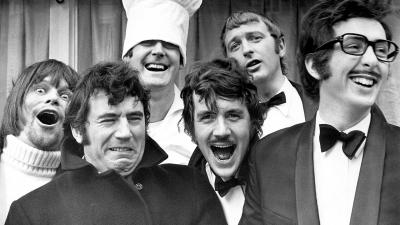
\includegraphics[width=0.8\linewidth]{python.jpg}
  \end{figure}
\end{frame}

\begin{frame}{Особенности языка Python}
  \begin{itemize}
    \item Высокоуровневый
    \item Интерпретируемый
    \item Динамически типизируемый
    \item Поддерживает ООП
  \end{itemize}
\end{frame}

\begin{frame}{Версии Python}
  \centering
  ``Python 2.x is legacy, \\
  Python 3.x is the present
  and future of the language'' \footnote[frame]{
    https://wiki.python.org/moin/Python2orPython3}
\end{frame}

\begin{frame}{Документация}
  \begin{enumerate}
    \item help()
    \item docs.python.org
    \item opennet.ru/docs/RUS/python/
  \end{enumerate}
\end{frame}

\begin{frame}[fragile]{Hello, world!}
  \begin{itemize}
  \item REPL:
    \begin{lstlisting}
python
>>> print("Hello, world!")
    \end{lstlisting}
  \item hello.py:
    \begin{lstlisting}[numbers=left]
#!/usr/bin/env python
print("Hello, world!")
    \end{lstlisting}

  \begin{minipage}{0.4\linewidth}
     \begin{lstlisting}[language=bash]
chmod +x hello.py
./hello.py
     \end{lstlisting}
   \end{minipage}
   \hfill or \hfill
   \begin{minipage}{0.4\linewidth}
     \vspace{3.5mm}
     \begin{lstlisting}[language=bash]
python hello.py
     \end{lstlisting}
   \end{minipage}

  \end{itemize}
\end{frame}

\begin{frame}{\texttt{python -c "import this"}}
\footnotesize{
Красивое лучше, чем уродливое. \\
Явное лучше, чем неявное. \\
Простое лучше, чем сложное. \\
Сложное лучше, чем запутанное. \\
Плоское лучше, чем вложенное. \\
Разреженное лучше, чем плотное. \\
Читаемость имеет значение. \\
Особые случаи не настолько особые, чтобы нарушать правила. \\
При этом практичность важнее безупречности. \\
Ошибки никогда не должны замалчиваться. \\
Если не замалчиваются явно. \\
Встретив двусмысленность, отбрось искушение угадать. \\
Должен существовать один --- и, желательно, \\
\hspace{20.6mm} только один --- очевидный способ сделать это. \\
Хотя он поначалу может быть и не очевиден, если вы не голландец. \\
Сейчас лучше, чем никогда. \\
Хотя никогда зачастую лучше, чем прямо сейчас. \\
Если реализацию сложно объяснить --- идея плоха. \\
Если реализацию легко объяснить --- идея, возможно, хороша. \\
Пространства имён — отличная штука! Будем делать их побольше!
}
\end{frame}

\begin{frame}{Литералы}
  \begin{itemize}
    \item A-Z, a-z, 0-9, \_
    \item Case sensitive
  \end{itemize}
\end{frame}

\begin{frame}{Базовые типы данных}
  \begin{itemize}
    \item Boolean
    \item Integer
    \item Float
    \item Complex
    \item String\footnote[frame]{
        Существуют различия в типах данных в разных версиях Python: \\
        https://docs.python.org/2.7/library/stdtypes.html \\
        https://docs.python.org/3.4/library/stdtypes.html}
  \end{itemize}
\end{frame}

\begin{frame}[fragile]{Базовые типы данных}
  \begin{lstlisting}[numbers=left]
#!/usr/bin/env python

logic   = True         # A boolean assignment
counter = 103          # An integer
miles   = 1000.0       # A floating point
cmplx   = 1 + 1j       # A complex
name    = "John"       # A string

print(logic, not logic)
print(counter, counter * miles)
print(miles, miles / counter, miles // counter)
print(cmplx, cmplx.conjugate())
print(name, "|".join(name))
\end{lstlisting}
\end{frame}

\begin{frame}[fragile]{Преобразование типов}
  \begin{lstlisting}[numbers=left]
type(x)
int(x[, base])
float(x)
complex(real[,imag])
str(x)
\end{lstlisting}
\end{frame}

\begin{frame}[fragile]{Операторы}
\begin{lstlisting}
+, -, *, /, %, **, //    # arithmetical
==, !=, <, >, >=, <=     # comparison
and, or, not             # logical
in                       # membership
is                       # identity
\end{lstlisting}
\end{frame}

\begin{frame}[fragile]{Пара слов про коллекции}
  \begin{itemize}
  \item<1-> List
    \begin{lstlisting}[numbers=left]
l = [1, 2]
l.append(3)
print(l)
l.append(l)
print(l)
    \end{lstlisting}
  \item<2-> Dict
    \begin{lstlisting}[numbers=left]
d = {"one": 1, "two": 2,}
d["three"] = 3
print(d)
del(d["two"])
print(d)
    \end{lstlisting}
  \end{itemize}
\end{frame}

\begin{frame}[fragile]{Примечания}
  \begin{itemize}
    \item \lstinline$'foo' == "foo"$

    \item Comment:
      \begin{lstlisting}
# This is a comment example.
      \end{lstlisting}

    \item Docstring:
      \begin{lstlisting}
"""
This is a docstring example.

It is used for documentation purposes.
"""
      \end{lstlisting}
  \end{itemize}
\end{frame}

\begin{frame}[fragile]{Условный оператор}
  \begin{lstlisting}[numbers=left]
x = int(raw_input("Please enter an integer: "))
if x < 0:
    x = 0
    print("Negative changed to zero")
elif x == 0:
    print("Zero")
elif x == 1:
    print("Single")
else:
    print("More")
  \end{lstlisting}
\end{frame}

\begin{frame}[fragile]{Оператор цикла for}
  \begin{lstlisting}[numbers=left]
words = ["cat", "window", "defenestrate"]
for w in words:
    print(w, len(w))
\end{lstlisting}
\end{frame}

\begin{frame}[fragile]{Функция range}
  \begin{lstlisting}[numbers=left]
print(range(5))
print(range(3,10))
print(range(3, 10, 2))
print(range(3, 10, -2))
\end{lstlisting}
\end{frame}


\begin{frame}[fragile]{Оператор цикла for}
  \begin{lstlisting}[numbers=left]
words = ["cat", "window", "defenestrate"]

for i in range(len(words)):       # ugly
    print(i, words[i])

for i, word in enumerate(words):  # much better
    print(i, word)
\end{lstlisting}
\end{frame}


\begin{frame}[fragile]{Оператор цикла for}
  \begin{lstlisting}[numbers=left]
for n in range(2, 10):
     for x in range(2, n):
         if n % x == 0:
             print(n, "equals", x, "*", n/x)
             break
     else:
         print(n, "is a prime number")
  \end{lstlisting}
\end{frame}

\begin{frame}[fragile]{Оператор цикла for}
  \begin{lstlisting}[numbers=left]
for num in range(2, 10):
    if num % 2 == 0:
         print("Found an even number", num)
         continue
    print("Found a number", num)
  \end{lstlisting}
\end{frame}

\begin{frame}[fragile]{Оператор цикла while}
  \begin{lstlisting}[numbers=left]
while True:
    pass
  \end{lstlisting}
\end{frame}

\begin{frame}[fragile]{Math module}
\begin{lstlisting}[numbers=left]
import math
dir(math)
help(math)
\end{lstlisting}
\end{frame}

\begin{frame}[fragile]{Задача <<поиск n-того числа Фибоначчи>>}
\begin{equation*}
  F_n = \left\{
    \begin{array}{l l}
      0 & \quad \text{при n = 0;}\\
      1 & \quad \text{при n = 1;}\\
      F_{n-1} + F_{n-2} & \quad \text{при n > 1.}
    \end{array} \right.
\end{equation*}
\end{frame}

\begin{frame}[fragile]{Задача <<поиск n-того числа Фибоначчи>>\footnote[frame]{
http://stackoverflow.com/questions/494594/how-to-write-the-fibonacci-sequence-in-python}}
\begin{lstlisting}[basicstyle=\footnotesize\ttfamily,numbers=left]
def fib(n):
    """ Return n-th number in Fibonacci sequence. """
    if n == 0: return 0
    elif n == 1: return 1
    else: return fib(n-1) + fib(n-2)

reqNumber = int(raw_input(
"Enter index of requested Fibonacci number: "))
print("Your number is:", fib(reqNumber))
\end{lstlisting}
\end{frame}

\begin{frame}{Задача <<n-тоe число Фибоначчи>>}
  \begin{itemize}
  \item Всегда ли эта программа работает корректно?
  \item Как оптимизировать процесс вычислений?
  \end{itemize}
\end{frame}

\begin{frame}{Домашнее задание}
  \begin{enumerate}
  \item Исправить ошибки
  \item Оптимизировать рекурсивную реализацию
  \item Написать нерекурсивную реализацию
  \item Сравнить производительность
  \end{enumerate}
\end{frame}

\begin{frame}{Спасибо за внимание!}
  \begin{itemize}
  \item https://github.com/budnyjj/courses\_python
  \item https://vk.com/budnyjj
  \item budnyjj@gmail.com
  \end{itemize}
\end{frame}
\end{document}